\documentclass{article}

% Language setting
\usepackage[spanish]{babel}

\usepackage[letterpaper,top=2cm,bottom=5cm,left=3cm,right=3cm,marginparwidth=1.75cm]{geometry}

% Useful packages
\usepackage{amsmath}
\usepackage{graphicx}
\usepackage[colorlinks=true, allcolors=blue]{hyperref}
\usepackage{amssymb}
\usepackage{fancyhdr}
\usepackage{lipsum}
\usepackage{multicol}
\usepackage{url}
\usepackage{float}

\pagestyle{fancy}

\fancyhf{}
\setlength{\headheight}{70pt}

% Definición del encabezado
\fancyhead[C]{%
    \begin{minipage}[c]{2.0cm}
        \centering
        
\includegraphics[width=2.0cm]{img/uta.png}
    \end{minipage}%
    \hfill
    \begin{minipage}[c]{8cm}
        \centering
        \small {\textbf{UNIVERSIDAD TÉCNICA DE AMBATO}} \\[0.1cm]
        \scriptsize \textit{FACULTAD DE INGENIERÍA EN SISTEMAS ELECTRÓNICA E INDUSTRIAL} \\[0.1cm]
        \scriptsize \textbf{CARRERA SOFTWARE - Base de Datos} \\[0.1cm]
        \scriptsize \textbf{CICLO ACADÉMICO: AGOSTO 2025 - ENERO 2026}
    \end{minipage}%
    \hfill
    \begin{minipage}[c]{2.0cm}
        \centering
        
\includegraphics[width=2.0cm]{img/fisei.png}
    \end{minipage}%
}

\begin{document}

\begin{center}
    {\large \textbf{INFORME DE TAREA}} \\
\end{center}

\section{Portada}
\begin{flushleft}
\begin{tabular}{ l l }
    \textbf{Tema:} & Prueba del Primer Parcial \\
    \textbf{Unidad de Organización Curricular:} & Profesional \\
    \textbf{Nivel y Paralelo:} & 4to Semestre ``B'' \\
    \textbf{Alumnos participantes:} & Molina Karen \\
    & Guatemal Bryan \\
    & Gisselle Espín \\
    & Benjarano Carlos \\
    \textbf{Asignatura:} & Base de Datos \\
    \textbf{Docente:} & Ing. Jose Ruben Caiza Caizabuano Mg. \\
\end{tabular}
\end{flushleft}

\section{Informe de la Tarea}

\subsection{Objetivos}

\subsubsection{General}
Desarrollar el esquema lógico de una base de datos para gestionar la información de cooperativas de transporte, socios, unidades, provincias, cantones, viajes, controles de calidad e incumplimientos, aplicando principios de diseño de bases de datos.

\subsubsection{Específicos}
\begin{itemize}
    \item Identificar las entidades, atributos y relaciones presentes en el caso planteado.
    \item Establecer las cardinalidades entre las entidades del sistema.
    \item Convertir el modelo conceptual en tablas y revisar las reglas de integridad correspondientes.
\end{itemize}

\subsection{Instrucciones}

Se desea crear una base de datos para controlar los viajes de las cooperativas de transporte hacia las diferentes ciudades del país.

De las cooperativas de transporte se conoce el código, nombre, dirección y teléfono. Una cooperativa tiene muchos socios, pero cada socio puede pertenecer únicamente a una cooperativa.

Un socio tiene muchas unidades o buses, pero cada unidad pertenece solamente a un socio. De cada socio se conoce la cédula, nombre, apellido, dirección, teléfono y fecha de nacimiento. De cada unidad o bus se conoce el número de disco (ID), marca, año, placa y capacidad de pasajeros.

Una provincia tiene muchos cantones, pero cada cantón pertenece solo a una provincia. De cada provincia se conoce el código, nombre y ubicación. De cada cantón se conoce el código, nombre y referencia geográfica.

Muchos buses viajan a muchos cantones. De cada viaje se conoce el número de viaje, la fecha y hora de salida, la fecha y hora de llegada, el costo del asiento y la cantidad de pasajeros que viajan.

A los buses se les realizan controles de calidad anuales. Un bus pasa varios controles y cada control se aplica a un solo bus. Del control se conoce un código, la fecha del control, el tipo de control, el identificador del funcionario responsable del control y el resultado del control, el cual puede ser aprobado o reprobado.

Un control puede tener muchos incumplimientos. De cada incumplimiento se conoce el identificador, la descripción y el nivel de gravedad de la novedad.

\textbf{Secuencia sugerida:}
\begin{enumerate}
    \item Lea el caso.
    \item Identifique entidades.
    \item Defina cardinalidades.
    \item Convierta a tablas.
    \item Revise integridad.
\end{enumerate}

Desarrolle hasta el esquema lógico y utilice herramientas acordes a la solución. Además, considere la siguiente figura para la presentación:

\begin{figure}[H]
    \centering
    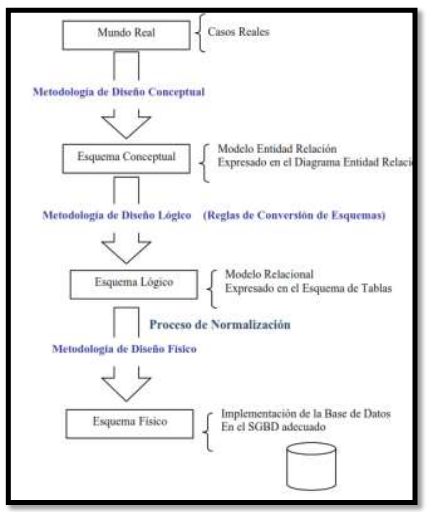
\includegraphics[width=0.55\textwidth]{img/metodologia.png}
    \caption{Metodología considerada para la presentación del desarrollo de la tarea.}
    \label{fig:metodologia}
\end{figure}

\subsection{Listado de equipos, materiales y recursos}

\textbf{Listado de equipos y materiales generales empleados en la tarea:}
\begin{itemize}
    \item Computadora o laptop.
    \item Documento guía proporcionado por el docente.
    \item Herramienta de modelado de bases de datos.
    \item Editor de texto para la elaboración del informe.
\end{itemize}

\textbf{TAC (Tecnologías para el Aprendizaje y Conocimiento) empleados en la tarea:}
\begin{itemize}
    \item[$\square$] Plataformas educativas
    \item[$\square$] Simuladores y laboratorios virtuales
    \item[$\boxtimes$] Aplicaciones educativas
    \item[$\square$] Recursos audiovisuales
    \item[$\square$] Gamificación
    \item[$\boxtimes$] Inteligencia Artificial
    \item Otros (Especifique): Herramienta de modelado de bases de datos
\end{itemize}

\subsection{Desarrollo de la Tarea (Actividades a Desarrollar)}

En esta sección se incorporará posteriormente el desarrollo detallado de la tarea, incluyendo la identificación de entidades, atributos, relaciones, cardinalidades, conversión a tablas y revisión de reglas de integridad, conforme a las indicaciones del caso planteado.

\subsection{Resultados obtenidos}

Como resultado de la actividad, se realizó el análisis del caso propuesto para el diseño de una base de datos orientada al control de viajes de cooperativas de transporte. Se identificó la necesidad de estructurar la información de cooperativas, socios, unidades, provincias, cantones, viajes, controles e incumplimientos dentro de un esquema lógico coherente y normalizado.

El desarrollo detallado de los resultados, junto con las tablas y figuras correspondientes, será incorporado en esta sección una vez concluida la fase de modelado.

\subsection{Habilidades blandas empleadas en la tarea}
\begin{itemize}
    \item[$\square$] Liderazgo
    \item[$\boxtimes$] Trabajo en equipo
    \item[$\boxtimes$] Comunicación asertiva
    \item[$\square$] La empatía
    \item[$\boxtimes$] Pensamiento crítico
    \item[$\square$] Flexibilidad
    \item[$\square$] La resolución de conflictos
    \item[$\boxtimes$] Adaptabilidad
    \item[$\boxtimes$] Responsabilidad
\end{itemize}

\subsection{Conclusiones}

El caso propuesto permitió identificar los elementos fundamentales necesarios para el diseño de una base de datos relacional aplicada al control de viajes de cooperativas de transporte. A partir del análisis realizado, se determinó que el sistema requiere una adecuada organización de entidades, atributos y relaciones para representar correctamente la realidad planteada.

Asimismo, se evidenció la importancia de definir cardinalidades y reglas de integridad antes de convertir el problema en un esquema lógico, ya que esto permite evitar redundancias y mejorar la consistencia de los datos dentro del modelo relacional.

\subsection{Recomendaciones}

Se recomienda desarrollar el modelo lógico utilizando una herramienta especializada de diseño de bases de datos, ya que esto facilita la representación ordenada de las tablas, claves primarias y claves foráneas.

También se recomienda revisar cuidadosamente las relaciones de uno a muchos y de muchos a muchos presentes en el caso, con el fin de construir un esquema lógico correcto, claro y acorde con las necesidades del problema planteado.

\subsection{Referencias}
Insertar las referencias bibliográficas empleadas aplicando la norma IEEE.

\vspace{-3em}
\renewcommand{\refname}{}
\bibliographystyle{ieeetr}
\bibliography{citas}

\subsection{Anexos}
Se podrán incorporar en esta sección las capturas del modelo conceptual, modelo lógico y cualquier evidencia del desarrollo realizado con la herramienta utilizada.

\vfill

\end{document}